\section{Method} \label{sec:method} 

In this section we will describe the method we have used to solve the Authorship
Verification problem presented. In general there are two methods of representing
each author. There is the instance based approach and the profile based
approach. In the instance based approach each author is represented by a set of
texts they have written while in the profile based approach they are represented
by the sum of the set of texts they have written. The instance based approach is
illustrated in Figure \ref{fig:instance_based} and the profile based approach is
illustrated in Figure \ref{fig:profile_based}.

\begin{figure}[htb]
    \centering
    \textbf{Instance Based Authorship Verification or Authorship Attribution}
    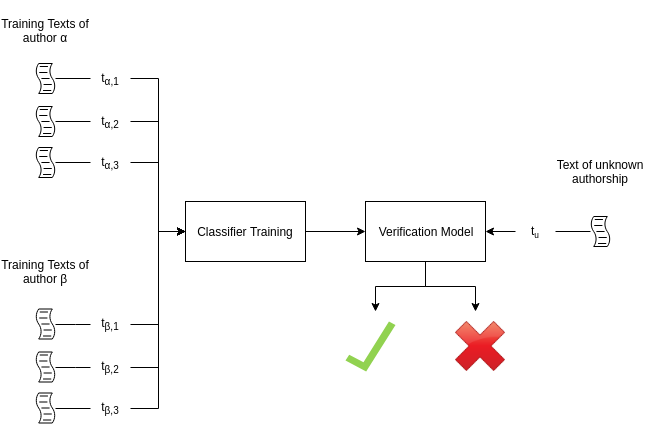
\includegraphics[scale=0.5]{./pictures/method/InstanceBased.png}

    \caption{Illustrate the typical instance based Authorship Verification or
    Authorship Attribution solution setup. Inspired by \cite{stamatos2009} a
    set of authors are given as input each with a set of texts. Some Machine
    Learning model is trained on the input texts and the model is used to
    predict an unknown text. }

    \label{fig:instance_based}
\end{figure}

\begin{figure}[htb]
    \centering
    \textbf{Profile Based Authorship Verification or Authorship Attribution}
    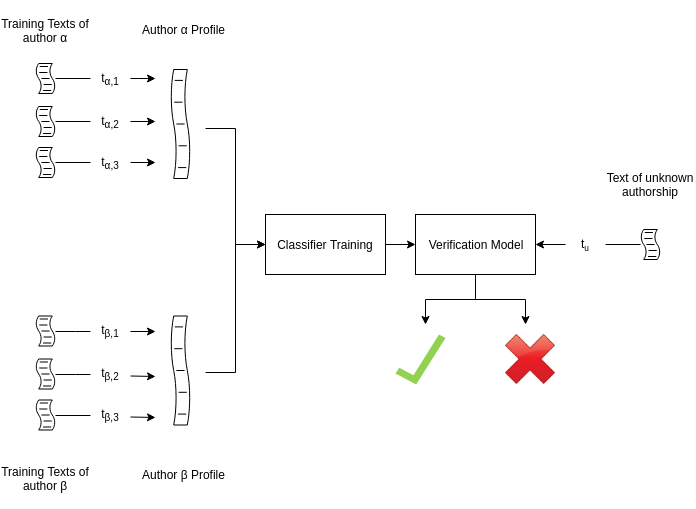
\includegraphics[scale=0.5]{./pictures/method/ProfileBased.png}

    \caption{Illustrate the typical profile based Authorship Verification or
    Authorship Attribution setup. Inspired by \cite{stamatos2009} the texts of
    each author are combined using some combination function such as an average
    or a concatenation. Those \textit{profiles} are then given to a Machine
    Learning model to train. The output is a model which is used to predict
    unknown texts. }

    \label{fig:profile_based}
\end{figure}

We will generally use the instance based approach. The reason we use an instance
based approach is that it allows us to use extra information from each single
text. For example writing style may change over time especially for secondary
school pupils that evolve very much in a short amount of time. Since we use an
instance based approach we are able to weight similarity to newer texts higher
than similarity to older texts.

There are also another split between methods that we consider. There are
generalizing and author specific models. In a generalizing model only a single
model is trained on data from multiple authors and are able to make predictions
about previously unseen authors. In the author specific model a separate model
has to be trained for each author and is not able to make predictions for
previously unseen authors. The generalizing model has several advantages, it
only has to be trained once and after that it can be used for everyone and
it can make use of big data since it can use data from several authors for
training. The author specific model has the advantage that it can better fit
to the specific quirks of a particular author since it is trained separately
for each author. The downside of the author specific approach is that a new
model has to be trained for each new author. We will focus on the generalizing
approach since it is easier to implement for MaCom as they only have to train a
model once.

As a unit of measuring the quality of our models, and how well they adhere to
95\% specificity constraint, we will also compute the number of \gls{TP}s,
\gls{TN}s, \gls{FP}s and \gls{FN}s, as was done in a project previously created
by us.\cite{US} In these problems we get,

\begin{itemize}
    \item a \gls{TP} whenever we answer \textit{True} and the texts are written
        by the same author,
    \item a \gls{TN} whenever we answer \textit{False} and the texts are
        \textbf{not} written by the same author,
    \item a \gls{FP} whenever we answer \textit{True} and the texts are
        \textbf{not} written by the same author,
    \item a \gls{FN} whenever we answer \textit{False} and the texts are written
        by the same author.
\end{itemize}

Given those definitions the \gls{TPR}, \gls{FPR}, \gls{TNR} and \gls{FNR}
describes.

\begin{description}
    \item[\gls{TPR}: ] The fraction of positives that we reported \textit{True}
        on i.e. the fraction of texts written by the same author that we say are
        written by the same author.
    \item[\gls{FPR}: ] The fraction of negatives that we reported \textit{True}
        on i.e. the fraction of texts written by different authors that we say
        are written by the same author.
    \item[\gls{TNR}: ] The fraction of negatives that we reported \textit{False}
        on i.e. the fraction of texts written by different authors that we say
        are written by different authors.
    \item[\gls{FNR}: ] The fraction of positives that we reported \textit{False}
        on i.e. the fraction of texts written by the same author that we say are
        written by different authors.
\end{description}

And they can be computed as,

\begin{align}
    TPR &= \frac{TP}{TP + FN}, \\
    FPR &= \frac{FP}{FP + TN}, \\
    TNR &= \frac{TN}{TN + FP}, \\
    FNR &= \frac{FN}{FN + TP}.
\end{align}

Using these definition we can also describe the accuracy measure we will be
reporting on throughout our experiments.

\begin{equation}
    \text{Accuracy} = \frac{TP + TN}{TP + FP + TN + FN}
\end{equation}


In the case of MaCom, we want to minimize the \gls{FNR} as much as possible, so
as to not wrongfully accuse anyone of not having written their assignment.
This however leaves out a equally important metric. While a low \gls{FNR}
is the goal, MaCom also wants to minimize the number of \gls{FN}s compared
to the total number of accusations made. This can be described as:
$$
\text{Accusation Error} = \frac{FN}{FN + TN}
$$
Our goal is also to keep this value under a certain threshold specified by MaCom.


\subsection{Baseline Methods}

In order to gauge the efficiency of our deep learning approaches, we have chosen
to implement some baseline methods. These methods were picked based on their
performance in a previous project written by us \cite{US}. Albeit that project
was only concerned with English texts provided by the \cite{pan:2015}, and
\cite{pan:2014} text forensics tasks, we hypothesize that the performance of
these approaches will perform just as well on Danish texts when being tuned for
the Danish language.


\subsubsection{Extended Delta Method}

One of the best performing methods of \cite{US} was the extended delta method.
As the name suggests the method extends the already existing delta method
described by \cite{evert2015towards}. The normal delta methods consists of first
extracting word frequencies from all texts and using these as the describing
features. After doing this to the entire sample space of texts, and applying a
linear transformation to their respective feature-sets, \gls{KNN} is then used
to determine the author of the introduced texts based on its closest neighbors
in the word-frequency feature-space. The extended delta method, simply expands
on the set of possible features to pick from, rather than being limited to only
using the word-frequencies of the text.


\subsubsection{Author Specific SVM}

Another algorithm used in \cite{US}. Heavily inspired by \cite{hansen2014}
starts out by fetching all texts known to be written by a specific author and an
equal number of texts known not to be written by that same author. It is upon
the feature-set extracted from these texts that a \gls{SVM} is trained, allowing
it to learn the specific author's writing style from the known texts supplied
and in contrast what the writing style of someone not him is. When a new text,
with disputed authorship is presented the hope is that the trained \gls{SVM}
will be able to determine if the author it was trained on, is in fact the author
of this new text as well.


\subsection{Deep Learning}

In this paper we will approach the authorship verification/attribution problem
using deep-learning. The term deep learning, was first introduced to
machine machine learning in 1989, and afterward to \gls{NN}'s in 2000. The terms
quickly became synonymous with \gls{NN}'s due to them being some of the more
efficient deep learning methods.\cite{Schmidhuber:2015}

With the inner workings of the brain used as the basis, a standard simple
\gls{NN} consists of a set interconnected processors, called neurons. Each of
these neurons has a real-valued activation associated with it, which activates
differently depending on the specific neuron. The input neurons activate through
perceiving the environment, or in other words, when it is fed data externally.
Other neurons are simply activated through the weighted activation of previous
neurons. More details regarding these weights will be presented later in the
paper.\cite{DBLP:journals/corr/Schmidhuber14}

\gls{NN}'s have been around since the 1940's. However, back then they were
merely variations of the linear regressors used at the time, and wasn't
very reminiscent of the Networks on can see today. It wasn't until the
late 1960's, early 70's, that networks comparable to the more modern
approaches surfaced. Examples of such early works, are the two publications
\cite{ivakhnenko1973cybernetic} and \cite{4308320}, which describe multi-layered
feed-forward supervised neural network architectures. While the work described
in \cite{4308320} was indeed one of the first cases of the modern \gls{NN},
actually getting the network to learn was still a problem, as the tweaking of
individual weights attributed to each neuron in the network wasn't trivial.
Little did they know, research to solve that problem was already in progress.
The basics of continuous \gls{BP} was initially described in 1960, in
\cite{Kelley1960}, quickly followed by a simpler approach which used only the
chain rule in 1962, \cite{DREYFUS196230}. It wasn't until 1970 that the modern
version of \gls{BP} was described, using automatic differentiation as its
basis. With this, the increase in research of usages of \gls{BP} increased the
following decades. As the computational power increased several 1000 folds in
the 90's and 2000's, so did the practical usage of \gls{BP}, and \gls{NN} in
general\cite{Schmidhuber:2015}. The real life application of \gls{BP}, will be
described in Section \ref{sec:BP}

Like with the history of authorship attribution, research in this area of
science picked up more interest, as we entered the modern computational age, and
with the introduction of the \gls{CNN}. \gls{CNN}s are based on the early work
described in \cite{TJP:TJP19681951215}. They showed that cats and monkeys visual
cortexes contain a set of neurons, each individually responding to a receptive
field, or area, of their field of view. Neighboring receptive fields all have a
certain amount of overlap, however in the end a cohesive view is created. This
is what paved the way for neocognition in 1980\cite{Fukushima1980}, the basis
of \gls{CNN}'s, which works in a very similar manner, looking at overlapping
subsections of data. These convolutional neurons however were rarely used alone,
but together with a down-sampling neuron such as Max Pooling introduced in
1993.\cite{Schmidhuber:2015}

\subsubsection{Neurons}\label{sec:neurons}

As mentioned previously a \gls{NN} consists of a collection of neurons. Each
neuron is a simplified mathematical model, which behaves much like neurons in
the brain would, receiving, processing and transmitting data/information. Each
neuron has a set of inputs called $x_i$ and a single output called $z_i$. The
neurons compute a weighted sum of its inputs and applies an activation function
$h$ to the weighted sum. The weights are called $w_i$. The function each neuron
computes is then,

\begin{equation}\label{eq:neuron}
    z_i = h\left(
        \sum_{i = 1}^d w_ix_i + w_0
    \right).
\end{equation}

One has the options to arrange the neurons in what is called layers, to achieve
a certain desired behavior, more details regarding these specific layers will
be explained in later chapters.
The training of a \gls{NN} consists of changing the weights applied at each
neuron, with the goal of modeling the relationships present in the data.

\subsubsection{Layers} \label{subsubsec:layers}

\gls{NN}'s are organized in layers. The first layer is called the input layer
and is connected directly to the input to the model and the last layer is called
the output layer and gives the output of the model. All layers in between are
called hidden layers. The input layer could for example be a layer of neurons
where each neuron is connected to a pixel in an input image. And the output
layer could consist of a single neuron that computes the probability that the
picture contained a cat. An example layered \gls{NN} are shown in Figure
\ref{fig:example_nn}.

\begin{figure}
    \centering
    \textbf{Example Neural Network}\par\medskip
    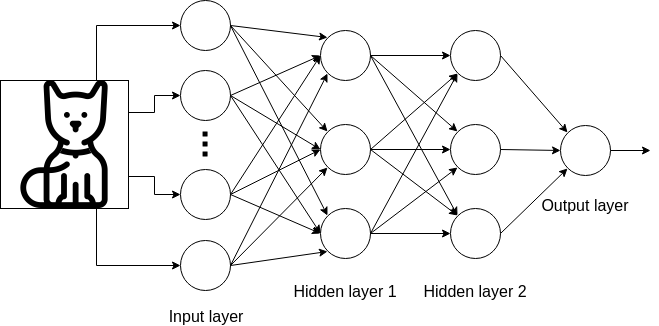
\includegraphics[width=\textwidth]{./pictures/method/example_neural_network.png}
    \caption{Example neural network that illustrates how neurons are organized
        into different layers with a special input layer and a special output
        layer. The neurons in the input layer are connected to individual pixels
        in an input image and the output layer is a single neuron computing the
        probability that the image contains a cat.}
    \label{fig:example_nn}
\end{figure}

There are different kinds of layers. Below is a non-exhaustive description of
different layers.

\begin{description}
    \item[Dense Layer:] In a dense layer the input of each neuron in the
        layer is connected to the output of every neuron in the previous layer.
        Each neuron in the layer computes a weighted sum of the outputs of the
        previous layers' neurons and applies an activation function. The weights
        for each of the neurons in the layer are different allowing each neuron
        to learn a different combination of the previous layer. An example
        of this can be seen in figure \ref{fig:example_nn}, where the hidden
        layers are Dense.
    \item[Convolutional Layer:] A convolutional layer is mainly used to extract
        position independent features from data. The convolution consist of a
        sliding window that slides over some input data and gives an output for
        each possible position of the input image. The sliding window uses the
        same weights in all the input and will therefore extract the same
        features from different locations if it is presented with the same
        input. The convolution computes a single output for each window
        position. The output is computed as the sum of the elementwise
        multiplication of the sliding window and the current part of the input
        it is looking at. Lets for example consider a two dimensional input,

        \begin{equation}
            I = \begin{pmatrix}
                1 & 1 & 1 & 0 \\
                1 & 0 & 0 & 1 \\
                0 & 1 & 0 & 1 \\
                0 & 0 & 1 & 0
            \end{pmatrix},
        \end{equation}

        and the convolutional filter,

        \begin{equation}
            w = \begin{pmatrix}
                1 & 0 & 0 \\
                1 & 0 & 0 \\
                0 & 1 & 0 \\
            \end{pmatrix}.
        \end{equation}

        Then we start the sliding window in the top left corner and compute the
        elementwise product of the matrices,

        \begin{equation}
            X = I_{1-3,1-3} \circ w =
            \begin{pmatrix}
                1 & 1 & 1 \\
                1 & 0 & 0 \\
                0 & 1 & 0
            \end{pmatrix} \circ
            \begin{pmatrix}
                1 & 0 & 0 \\
                1 & 0 & 0 \\
                0 & 1 & 0
            \end{pmatrix} =
            \begin{pmatrix}
                1 & 0 & 0 \\
                1 & 0 & 0 \\
                0 & 1 & 0
            \end{pmatrix},
        \end{equation}

        to then compute the final value we take the sum of all the elements in
        that matrix,

        \begin{equation}
            \sum_{i,j} X_{i,j} = 1 + 0 + 0 + 1 + 0 + 0 + 0 + 1 + 0 = 3.
        \end{equation}

        We then slide the window one to the right and repeat the same process,

        \begin{equation}
            X = I_{2-4,1-3} \circ w =
            \begin{pmatrix}
                1 & 1 & 0 \\
                0 & 0 & 1 \\
                1 & 0 & 1
            \end{pmatrix} \circ
            \begin{pmatrix}
                1 & 0 & 0 \\
                1 & 0 & 0 \\
                0 & 1 & 0
            \end{pmatrix} =
            \begin{pmatrix}
                1 & 0 & 0 \\
                0 & 0 & 0 \\
                0 & 0 & 0
            \end{pmatrix},
        \end{equation}

        and the final value,

        \begin{equation}
            \sum_{i,j} X_{i,j} = 1.
        \end{equation}

        We keep sliding the window right until we run out of input. After that
        we go back to the left and go one row down. We continue the process for
        all the input and we end up with the matrix,

        \begin{equation}
            O = \begin{pmatrix}
                \sum_{i,j} \left( I_{1-3,1-3} \right)_{i,j} &
                \sum_{i,j} \left( I_{2-4,1-3} \right)_{i,j} \\
                \sum_{i,j} \left( I_{1-3,2-3} \right)_{i,j} &
                \sum_{i,j} \left( I_{2-4,2-3} \right)_{i,j}
            \end{pmatrix} = \begin{pmatrix}
                3 & 1 \\
                1 & 2
            \end{pmatrix}.
        \end{equation}

        It can be seen that the output size is smaller than the input size.
        To prevent that the input can be padded with some value. A normal choice
        is zero padding. For the above input that would result in,

        \begin{equation}
            \begin{pmatrix}
                1 & 1 & 1 & 0 \\
                1 & 0 & 0 & 1 \\
                0 & 1 & 0 & 1 \\
                0 & 0 & 1 & 0
            \end{pmatrix} \xrightarrow{\text{zero padding}}
            \begin{pmatrix}
                0 & 0 & 0 & 0 & 0 & 0 \\
                0 & 1 & 1 & 1 & 0 & 0 \\
                0 & 1 & 0 & 0 & 1 & 0 \\
                0 & 0 & 1 & 0 & 1 & 0 \\
                0 & 0 & 0 & 1 & 0 & 0 \\
                0 & 0 & 0 & 0 & 0 & 0
            \end{pmatrix}.
        \end{equation}

        The sliding length can be different than one and is usually referred to
        as stride. The weights the convolutional window uses are learnable and
        is updated via gradient descent. Certain convolutional filters can be
        used for edge detection and blurring the input. Some examples of
        different convolutional kernels applied to a grayscale image are shown
        in Figure \ref{fig:convolution_example}.

        \begin{figure}
            \centering
            \textbf{Examples of different convolutional kernels}\par\medskip
            \begin{tabular}{ccc}
                \textbf{Original} & \textbf{Kernel} & \textbf{Result} \\
                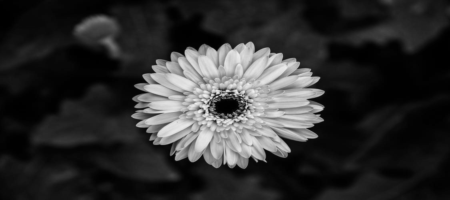
\includegraphics[width=0.3\textwidth]{./pictures/method/original_convolution.png} &
                \begin{minipage}{6cm}
                    \begin{equation*}
                        \begin{pmatrix}
                            1 & 0 & -1 \\
                            0 & 0 & 0  \\
                            -1 & 0 & 1
                        \end{pmatrix}
                    \end{equation*}
                \end{minipage}
                    &
                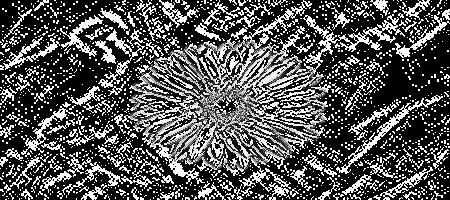
\includegraphics[width=0.3\textwidth]{./pictures/method/edge_detect_convolution.png} \\

                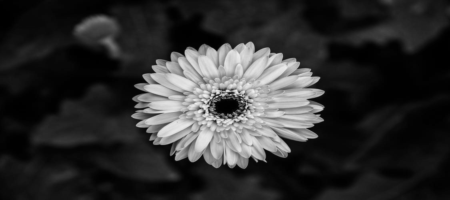
\includegraphics[width=0.3\textwidth]{./pictures/method/original_convolution.png} &
                \begin{minipage}{6cm}
                    \begin{equation*}
                        \frac{1}{16}\begin{pmatrix}
                            1 & 2 & 1 \\
                            2 & 4 & 2  \\
                            1 & 2 & 1
                        \end{pmatrix}
                    \end{equation*}
                \end{minipage}
                    &
                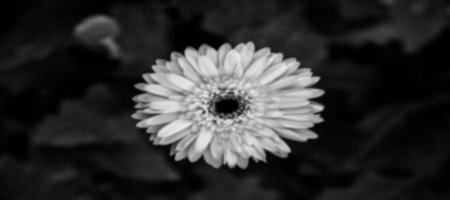
\includegraphics[width=0.3\textwidth]{./pictures/method/blurred_convolution.png} \\

                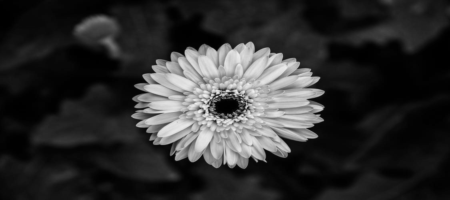
\includegraphics[width=0.3\textwidth]{./pictures/method/original_convolution.png} &
                \begin{minipage}{6cm}
                    \begin{equation*}
                        \begin{pmatrix}
                            0  & -1 & 0  \\
                            -1 & 5  & -1 \\
                            0  & -1 & 0
                        \end{pmatrix}
                    \end{equation*}
                \end{minipage}
                    &
                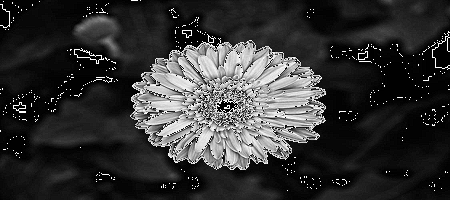
\includegraphics[width=0.3\textwidth]{./pictures/method/sharpened_convolution.png}
            \end{tabular}
            \caption{Examples of convolutional kernels applied to an image. The
                first kernel is an edge detect kernel, the second a blurring
                kernel and the third a sharpening kernel.}
            \label{fig:convolution_example}
        \end{figure}

        % TODO: Show example from text.
        % TODO: Maybe also explain different filters here.

    \item[\gls{LSTM} Layer:] TODO
    \item[\gls{GRU} Layer:] TODO

    \item[Embedding:] The Embedding layer is a layer that maps a value into a
        continuous vector space. Given a sequence of integers it uses the
        weights associated with the layer, to map that singular value to a
        vector of predetermined size. This can be done on any sort of data, as
        longs as it is encoded as a sequence of integers. In \gls{NLP}
        circumstances, this can be applied to characters or words for example,
        where each element in the sequence is firstly encoded as an integer
        value, and then fed to the embedding layer, which maps it to the
        continuous vector space. The hope with using a layer such as this, that
        characters for example, get mapped to a point close to other
        similar characters. In addition it also adds another trainable layer to
        optimize on.

    \item[Max Pooling Layer:] TODO.
\end{description}

\subsubsection{Back-Propagation}\label{sec:BP}

The neural network learns by updating the weights in the network. The weights
are updated using \gls{BP}. The process can be split into three distinct steps
which are continuously repeated:

\begin{enumerate}
    \item Feed Forward,
    \item Back Propagate, and
    \item Update Weights.
\end{enumerate}

% TODO: The gradient does not point the minimum. It points towards the maximum
% which is why we take a step in the opposite direction of the gradient.
% Furthermore it does not necessarily point towards the maximum. It only points
% in the direction which is "up" if we take an infinitesimally small step in
% that direction which is why you "zigzag" towards the goal and don't go in a
% strait line.
%
% TODO: Maybe refer to where we are "looking at the structure of our network".
%
% TODO: Rewrite sentence "The weights and the biases of the network that
% produces the output it computes its cost based on.".
%
% TODO: "In our case the bias is just, and as such, ...". What is the bias just?
The goal of these three steps is to minimize the overall cost of the network.
The cost refers to the loss we end up with. In order to do so, we take a step
in the direction of the negative gradient as the gradient points to where the
minimum cost can be found. Looking at the structure of our network, we can
quickly identify the error function being dependent on 2 values. The weights
and the biases of the network that produces the output it computes its cost
based on. In other words we have to determine the partial derivative of the
cost function with respect to the weights and the biases of the network (In our
case the bias is just, and as such, isn't relevant in this context due to is be
differentiated out).

\begin{lemma}[Chain Rule]
\label{lemma:chainrule}

    If functions \textbf{f} and \textbf{g} er both differentiable and
    \textbf{F} is the composite function defined by $F(x) = f(g(x))$,
    then $F' = f'(g(x)) \cdot g'(x)$,

\end{lemma}

But before actually being able to do so, we have took look at a neural network
for what it is, which is a series of functions calling each other in a recursive
manner, applying Equation \ref{eq:neuron} at each step of the way. As such we
seek the assistance of the chain rule (Lemma. \ref{lemma:chainrule}), a simple
network for example purposes (Figure \ref{fig:simple_NN}), and an error
function,

% TODO: Maybe use i as index variable instead of x. Also shouldn't it be y_x
% like it is \hat{y}_x?
$$
E = \frac{1}{2N}\sum_{x=1}^N(\hat{y}_x - y(x))^2.
$$

Where N is the total number of training samples, $\hat{y}$ is the predicted
result, and $y$ is the correct one. For simplicity's sake, we chose to focus
on a single sample. When this sample is run through the network(Step 1) seen
in Figure \ref{fig:simple_NN}, some things changes. Firstly, we only a single
sample, so the error can be rewritten to,

$$
E = \frac{1}{2}(\hat{y} - y)^2.
$$

Additionally, the network only has one neuron per layer and a bias of 1, so
we can rewrite the neuron function from Equation \ref{eq:neuron} to,

\begin{equation}\label{eq:neuron:small}
    \hat{y} = z_i = h_i\left(
        w_ix + 1
    \right).
\end{equation}

Where i denotes the index of the layer in which this computation happens. This
can be further rewritten to include the fact that $x$ is in fact the output of
the previous layer.

\begin{align}
    z_i = h_i\left(
        w_iz_{i-1} + 1
    \right)
\end{align}

For easy reference we give the input of the activation function a name,

\begin{equation}\label{eq:k_small}
k_i = w_iz_{i-1}+1.
\end{equation}

% TODO: Positively influences sound like the cost function increases which is
% the opposite of what happend.
The scenario is that we have performed step 1, and passed the sample through the
network. Step 2 (Back Progropagation) seeks to find the partial derivative of
the cost function $E$, and each weight of the network, to allow for each weight
to step in the direction that positively influences the cost of the network.
Starting out, this is to be done to the output node of the network. As such we
want to compute:

$$
\frac{\partial E}{\partial w_{L_N}}
$$

Which with all variables switched our is computed as such:

% TODO: Why is it now w_L instead of w_{L_N}?
\begin{align}
\frac{\partial E}{\partial w_{L}} &= \frac{\partial}{\partial w_{L}}\left(\frac{1}{2}(\hat{y} - y)^2\right) &\\
&= \frac{\partial}{\partial w_{L}} \left(\frac{1}{2}(z_L - y)^2\right) & \text{Substitute $\hat{y}$, as per equality \eqref{eq:neuron:small}}\\
&= \frac{\partial}{\partial w_{L}} \left(\frac{1}{2}(h_L(w_{L}z_{L-1} + 1) - y)\right) & \text{Further substitute}\\
&= \frac{\partial}{\partial w_{L}} \left(\frac{1}{2}(h_L(k_L) - y)\right) & \text{Use equality \eqref{eq:k_small} to simplify}\\
&= \frac{\partial}{\partial w_{L}} \left(E(h_L(k_L))\right) & \text{Substitute with E}\\
&= \frac{\partial E}{\partial h_L}\frac{\partial h_L}{\partial k_L}\frac{\partial k_L}{\partial w_{L}} & \text{Application of Lemma \ref{lemma:chainrule}}
\end{align}

% TODO: "matrix comprised of all the partial derivatives". Is this the gradient?
% If yes why not write that?
This reveals the partial derivatives dependence on the output of the former
layer of the network. As such, back propagation propagates the partial
derivative back throughout the network, getting the partial derivative at each
node. Using the final cost, we are then able to determine the desired weight
change at this node. After averaging the desired changes over all the training
samples, the weights are updated (Step 3), by stepping in the negative direction
of the matrix comprised of all the partial derivatives computed, mulitiplied by
a pre-determined step-size.

These three steps Feed-Forward, Back-Propagate and update weights are repeated
throughout the training cycle of the neural networks, so as to optimize the
weights after each full iteration on the training set. As is to be expected
this algorithm as very expensive computationally. For this reason in pratice,
a method called batching is used. This method, shuffles and split the training
dataset up into smaller batches. These batches are then run through the network
one at a time, performing back-propagation after each run-through. This results
in the gradient not being as accurate after each batch, but this introduced
inaccuracy is negligible compared to the computational time won.


\begin{figure}
\centering
\begin{neuralnetwork}[height=1]
    \newcommand{\nodetextclear}[2]{}
    \newcommand{\nodetextx}[2]{$x_#2$}
    \newcommand{\nodetexty}[2]{$y_#2$}
    \inputlayer[count=1, bias=false, title=$L-3$, text=\nodetextclear]
    \hiddenlayer[count=1, bias=false, title=$L-2$, text=\nodetextclear] \linklayers
    \hiddenlayer[count=1, bias=false, title=$L-1$, text=\nodetextclear] \linklayers
    \outputlayer[count=1, title=$L$, text=\nodetextclear] \linklayers
\end{neuralnetwork}
\caption{A simple single neuron per layer, neural network. Where $L$ describes
the layer, and $N$ notes the total number of layers in the network. The green
node is the input layer, and the red is the output}
\label{fig:simple_NN}
% TODO: N is not in the figure so maybe it doesn't have to be in the caption.
\end{figure}


\subsubsection{Activation Functions}
The activation function $h$, used at each neuron, defines the output of the
node given a certain input. A simple example of this would be computer chip
circuit, which can be seen as a series of activation functions outputting 0 or
1 depending on their input. This activation function would be a linear one.
When applying activation functions to neurons in \gls{NN}s, they are usually
non-linear, as it allows for the computation of more complex problems using a
smaller amount of neurons, relative to usage of a linear activation function,
as they allow for the universal function approximation, a point also made by
\cite{6797088}

A plot of different activation functions is shown in Figure
\ref{fig:activation_functions}.

\begin{figure}
    \centering
    \textbf{Activation Functions}\par\medskip
    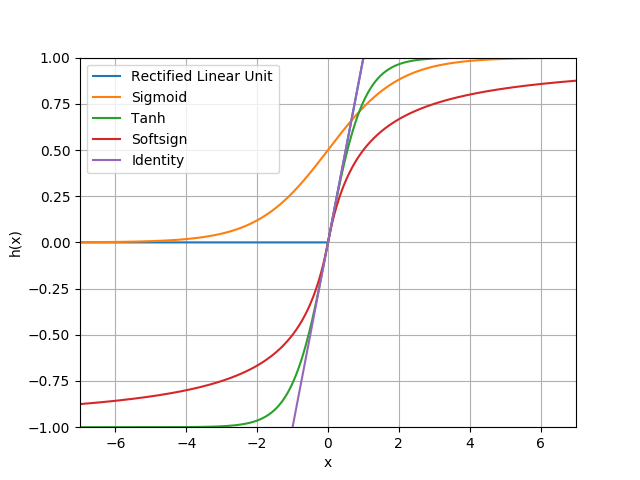
\includegraphics[width=0.5\textwidth]{./pictures/method/activation_functions.png}
    \caption{Different activation functions that can be used in neural
        networks.}
    \label{fig:activation_functions}
\end{figure}

Each activation function has its pros and cons. We mainly made use of the
\gls{ReLu} activation function in the hidden layers of our networks. The
reason for this selection is its general purpose use. When selecting an
activation function for your neurons, the best function would be the one which
best approximates the underlying function. Without a good idea as to what
that function might be, \gls{ReLu} is a good starting point. Its simplicity
provides a quick computation time, and its below zero limitation means that a
large portion of the network won't be activating, resulting in an even smaller
computation time. In addition to that, the derivative of the function is 1
in the case of a positive input, resulting in the \gls{BP} loss having equal
influence throughout the network. In the case of other activation functions,
this might not be the case, resulting in an altering of the error as we
propagate backwards through the network. This could lead to a big error in the
deeper layers not reaching the shallow layers of the network. This property of
the \gls{ReLu} activation function, does however not come without its costs.
If the learning rate of the network isn't configured correctly, a \gls{ReLu}
activated neuron might be blasted with a gradient so large, that it never
reaches a point of activation again. In other words, the neuron "dies". As
such, one can risk a network containing a lot of dead non-activation neurons,
thus greatly decreasing its quality. On the other hand the sigmoid function,
doesn't allow its neurons to die. It can become victim to saturation. In
the case of weight being too small or too high, the output values will be
placed at the far ends of the sigmoid range of values. At this point the
gradient is incredibly small, meaning that the contribution that neuron now has
is negligible. This neuron is now only a strain on the network, slowing it
down through its activation, but contribution nothing, a problem \gls{ReLu}
does not have. Its based on these considerations we chose the \gls{ReLu}
activation function, leaving us the task of properly selecting our learning
rate.\cite{JiYan, AndrejKarpathy, AvinashSharmaV}

As the activation function of our output neurons we have generally
used the softmax function. The softmax function is shown in Figure
\ref{fig:softmax_activation}. The function is defined as

\begin{equation}
    h(x_i) = \frac{e^{x_i}}{\sum_{k=1}^n e^{x_k}}, \text{for $i = 1 \dots n$}.
\end{equation}

The softmax function takes any vector $x \in \mathbb{R}^n$ and returns a vector
$y \in (0, 1)^n$. Where the sum of the output vectors elements will be equal to
1. The function is therefore great at constructing a probability distribution
based on an input vector. Each individual value in the vector get a high
probability if the value is high and a low probability if the value is low.
Therefore the function is often used at the end of networks to get the
probability of each class in a classification problem.

\begin{figure}
    \centering
    \textbf{Softmax Activation Function}\par\medskip
    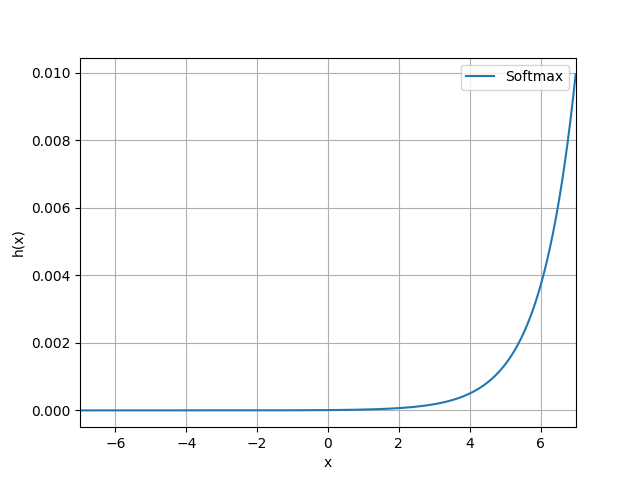
\includegraphics[width=0.5\textwidth]{./pictures/method/softmax_function.png}
    \caption{The softmax activation function.}
    \label{fig:softmax_activation}
\end{figure}

\subsubsection{Siamese Networks}

Classical machine learning approaches for text analysis and all our baseline
methods are based on handcrafted feature sets. Deep learning has shown
promising results in extracting features from raw images and raw text
\cite{hongxiaosunyuan}. We wanted to use deep learning to automatically learn
features from a large amount of data. At the same time we want to solve the
MaCom problem. Siamese neural networks are as described earlier networks that
compares two inputs. The networks has been used by \cite{Koch2015SiameseNN},
\cite{NIPS1993_769} and \cite{qian:2018} for comparing text, images and
signatures. \cite{qian:2018} use a Siamese network but with no convolutions and
a distance function on top for text analysis while \cite{Koch2015SiameseNN}
used a Siamese network with convolutions and fully connected network on top for
image analysis. Our approach is to use convolutions in the Siamese network to
learn important features from the texts. We also use a fully connected network
on top of the convolutional layers to learn from the features the convolution
extracted. An example of this architecture can be seen in Figure
\ref{fig:siamese_example}.

\begin{figure}
    \centering
    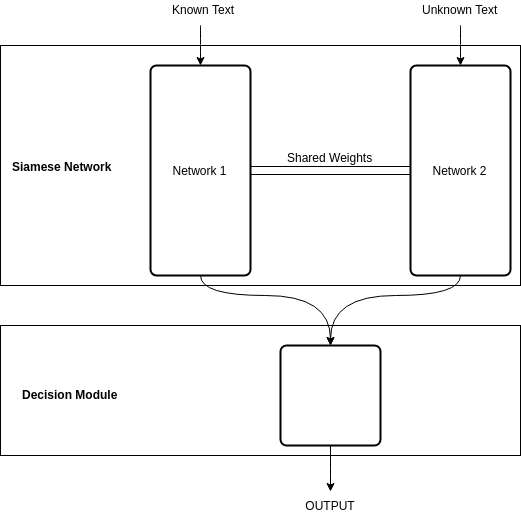
\includegraphics[scale=0.5]{./pictures/method/Siamese.png}
    \caption{The basic architecture of a Siamese neural network, which takes in
        two sources of data, and runs it through two parallelle networks,
        sharing their weights at each layer}
    \label{fig:siamese_example}
\end{figure}

The network will take two inputs, a text $t_k \in T_\alpha$ and a text $t_u
\in T_\beta$. The network will then try to figure out whether $\alpha =
\beta$. The convolutions in the network will look at $n$ characters at a
time and give an output. Therefore the convolutional layers will be able to
learn important n-grams and extract a representation of $t_k$ and $t_u$. This
representation will be given to some dense layers which will learn how to
compare the feature-sets extracted. The Siamese part of the network is the
convolutional part of the network which will share weights when extracting
n-grams from the two texts.

The final output of the network will be a probability that $\alpha = \beta$.
Since the MaCom dataset consist of multiple known texts per author and this
network architecture only compares two texts we define a separate system for
making the final prediction.

\subsection{Prediction System}

In the MaCom problem we are given a set of texts for each author so we can make
use of multiple texts when making our predictions. We can also use metadata
about the individual texts to make our prediction. An advantage of using
multiple texts for each author to make a prediction is that outliers will be
averaged out.

\begin{definition}[Prediction System]

    \label{def:prediction_system}

    Our prediction system is a function $P:f, w, \alpha, t_{unkown}, \theta
    \rightarrow \{0, 1\}$ where $f$ is a function taking two texts and giving
    the probability that the texts are written by the same author, $\alpha$
    is an author, $t_{unknown}$ is a text of unknown authorship, $w:T_\alpha
    \rightarrow [0,1]$ is a function where $\sum_{t_{known} \in T_\alpha}
    w(t_{known}) = 1$ and $\theta \in [0,1]$. The prediction system then
    returns,

    \begin{equation}
        P(f, w, \alpha, t_{unkown}, \theta) = \begin{cases}
            1 & \text{if } \sum_{t_{known} \in T_\alpha} w(t_{known})
                f(t_{known}, t_{unkown}) > \theta \\
            0 & \text{otherwise}.
        \end{cases}
    \end{equation}

\end{definition}

That is the prediction system returns 1 if the weighted average of the
probability that $t_{unknown}$ is written by the same author as $t_{known}$ for
each $t_k \in T_\alpha$ is greater than the threshold $\theta$ and 0 otherwise.

The $f$ parameter can be anything that takes two texts and returns a
probability. We are going to present several different networks that can be used
as $f$ as they will take two texts and end with a softmax layer that outputs a
probability distribution.

The $w$ parameter in the prediction system can be used to weigh the known texts
differently. We are going to try several different weight functions that weigh
texts based on metadata such as the time they were written and the length of
the texts. The only constraint on a weight function $w$ is that $\sum_{t \in
T_\alpha} w(t) = 1$. We will ignore that constraint in the following definitions
of weight functions. Any function $w: T_\alpha \rightarrow \mathbb{R}^+$ that
does not follow the constraint can be transformed into a version
$w^*: T_\alpha \rightarrow [0,1]$ that does follow the constraint where
$w^*(t) = \frac{w(t)}{\sum_{t \in T_\alpha} w(t)}$. We can therefore define the
weight functions $w$ while ignoring the constraint but use $w^*$ as the actual
weight function in the prediction system.

The most obvious weighing scheme is to just use a uniform
weighting. That way we simply take an average of the predictions of our networks
over the different texts an author has written.

\begin{definition}[Uniform Weighing]

    The uniform weight function $w_\mathcal{U}: T_\alpha \rightarrow \{1\}$ is
    defined as,

    \begin{equation}
        w_\mathcal{U}(t) = 1
    \end{equation}

\end{definition}

The uniform weight function does not use any information we know about the
texts. It is mostly part of our weight functions as a baseline to make sure we
don't make any weight functions that are worse than a simple uniform weighing.
Our other weight functions makes use of metadata we know about the texts. As an
example we have a timestamp of when a text was turned in to the MaCom servers.
We therefore know when the text was written and we assume that newer texts will
better reflect the current writing style of a student than older texts. We
have therefore defined several weight functions using the times the texts was
written. Let $\tau: T_\alpha \rightarrow \mathbb{N}$ be the function returning
the number of months between when the newest text $t \in T_\alpha$ and the
text it is given were turned in where a month is considered 30 days. Our time
based weight function are then defined as,

\begin{definition}[Exponential Dropoff]

    The exponential dropoff function $w_e: T_\alpha \rightarrow [0, 1]$ is
    defined as,

    \begin{equation}
        w_e(t) = e^{-\lambda \tau(t)}
    \end{equation}

\end{definition}

The $\lambda$ parameter in that weight function can be used to control how
important the newer texts are. When $\lambda = 0$ the Exponential Dropoff is
equivalent to the Uniform Weighing and as $\lambda \rightarrow \infty$ more
weight is given to the latest text. We have shown the weights given to different
assignments for different $\lambda$ values in Figure \ref{fig:weights}.

\begin{figure}
    \centering
    \textbf{Exponential Dropoff Weights}\par\medskip
    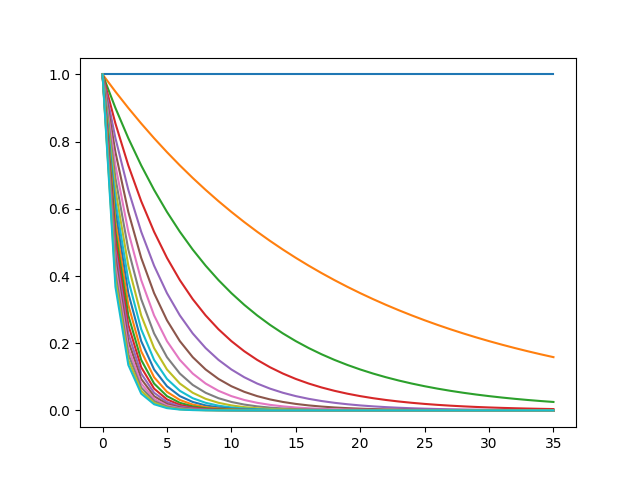
\includegraphics[width=0.49\textwidth]{./pictures/method/weights.png}
    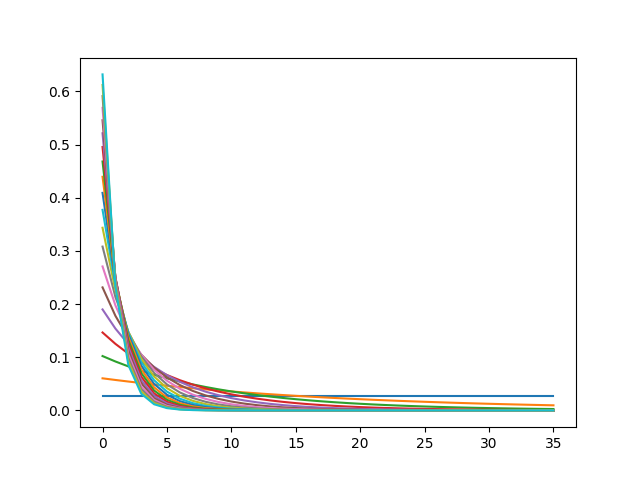
\includegraphics[width=0.49\textwidth]{./pictures/method/weights_normalized.png}
    \caption{Illustrate the Exponential Dropoff weight function for different
        values of lambda. We apply the weight function to the numbers $0, 1,
        \dots, 35$ since a typical student will attend high school for 3 years
        (36 months). On the left the pure output of the weight function $w_e$ is
        shown and on the right the normalized weights $w^*$. We wary $\lambda$
        from 0 to 1 with step size 0.05.}
    \label{fig:weights}
\end{figure}

%TODO: Define a weight function that also looks at the length of the texts.

The $\theta$ parameter in the prediction system determines when we consider an
unknown text to be written by an author. The natural choice for $\theta$ is 0.5
since that is what the network use when it computes the loss of each training
sample. However the $\theta$ parameter can be used to enforce how sure we have
to be of a decision to accuse an author of not having written an assignment. As
described earlier MaCom does not want to accuse innocent students of cheating.
That means that it is very important to MaCom to minimize the number accusation
error. We can use the $\theta$ parameter to control that error. Hopefully the
\gls{FN}s generally end up with a value closer to 1 than the \gls{TN}s. If that
is the case then lowering $\theta$ value will lower the fraction since there
will be fewer \gls{FN}s. That might lower the overall accuracy of the prediction
system but will make sure that at few students as possible are falsely accused.
